\documentclass[journal, 12pt, onecolumn, draftclsnofoot]{IEEEtran}
% \documentclass[10pt,conference]{IEEEtran} %INFOCOM 20'
\usepackage{amsfonts}
\usepackage{amssymb}
\usepackage{amsmath}
\usepackage[linesnumbered,vlined,ruled]{algorithm2e}
\usepackage{algorithmic}
\usepackage{amsthm}
\usepackage{array}
\usepackage[usenames]{color}
\usepackage{epsfig}
\usepackage{epstopdf}
\usepackage{extarrows}
\usepackage{graphicx} 
\usepackage{graphics}
\usepackage{amsmath,amsfonts,amssymb,mathrsfs}
\usepackage{mathtools}
\usepackage[dvipsnames]{xcolor}
\usepackage{dcolumn}
\usepackage[utf8]{inputenc}
\usepackage{soul}
\usepackage{array}
\usepackage{tabulary}
\graphicspath{ {./images/} }

% \IEEEoverridecommandlockouts

\newcommand{\revise}{\color{black}}
\newcommand{\revisesec}{\color{blue}}
\newcommand{\fixit}[1]{{\leavevmode\color{red}(#1)}}
\newcommand{\comments}[1]{{\leavevmode\color{blue}#1}}
\newcommand{\deny}[1]{}
\newcommand{\needref}[1]{\text{[#1]}}
%---------------------------------------------------------------%
\newcommand{\eq}{=}
\newcommand{\domZ}{\mathbb{Z}_{*}}
\newcommand{\domP}{\mathbb{Z}_{*}}
\newcommand{\vecOne}{\mathbf{1}}
\newcommand{\ind}{\mathbf{I}}
\newcommand{\mat}{\mathbf}
\newcommand{\Poisson}{\text{Poisson}}
\newcommand{\Bernoulli}{\text{Bernoulli}}
\newcommand{\define}{\triangleq}
\newcommand{\leadto}{\Rightarrow}
\newcommand{\vecG}{\boldsymbol}
\renewcommand{\vec}{\mathbf}
\DeclarePairedDelimiter{\set}{\{}{\}}
\DeclarePairedDelimiter{\norm}{|}{|}
\DeclarePairedDelimiter{\Inorm}{\|}{\|_1}
\DeclarePairedDelimiter{\Paren}{\bigg(}{\bigg)}
\DeclarePairedDelimiter{\Bracket}{\bigg[}{\bigg]}
\DeclarePairedDelimiter{\Brace}{\bigg\{}{\bigg\}}
%---------------------------------------------------------------%
\newtheorem{Definition}{Definition}
\newtheorem{Problem}{Problem}
\newtheorem{Lemma}{Lemma}
\newtheorem{Theorem}{Theorem}
\newtheorem{Algorithm}{Algorithm}
\newtheorem{Policy}{Policy}
\newtheorem{Scheme}{Scheme}
\newtheorem{Scenario}{Scenario}
\newtheorem{Assumption}{Assumption}
\newtheorem{Proposition}{Proposition}
\newtheorem{Remark}{Remark}
\newtheorem{Solution}{Solution}
\newtheorem{Baseline}{Baseline}
\newtheorem{Example}{Example}
\newtheorem{Corollary}{Corollary}
\newtheorem{Model}{Model}

\begin{document}
	
	\title{
		Joint Resource Scheduling for \deny{Heterogeneous} Communication and Computation Tasks in 5G C-RAN
	}
	\author{
        \IEEEauthorblockN{
            Yifei Sun,
            Yuncong Hong%,
            % Rui Wang,
            % Haisheng Tan,
            % Francis C.M. Lau
        }
        % \IEEEauthorblockA{\IEEEauthorrefmark{1}
        %     Department of Electrical and Electronic Engineering, Southern University of Science and Technology, Shenzhen, China \\
        % }
        % \IEEEauthorblockA{\IEEEauthorrefmark{2}
        %     Department of Computer Science, The University of Hong Kong, Hong Kong, China \\
        % }
        % \IEEEauthorblockA{\IEEEauthorrefmark{3}
        %     LINKE Lab, University of Science and Technology of China, Hefei, China \\
        % }
    }%
	\maketitle

\section{Introduction}
\begin{enumerate}
	\item C-RAN is the future, where functions of BBUs are implemented in a centralized and virtualized way;
	\item \fixit{Two concerns are not checked yet: a) how to assess resource requirement and evaluate tolerance of DT task? b) how to queue and perform selection action? }
	\item In this paper, we propose a novel framework where both BBU tasks and general edge computing tasks are processed simultaneously in a homogeneous edge cloud with general-purposed processors.
	\item By applying resource split between vBBU and vMC, the resource split between DT and CT is implemented. \fixit{So, why not just split computation resource for DT and CT?} 
\end{enumerate}

\begin{figure*}[htb!]
	\centering
	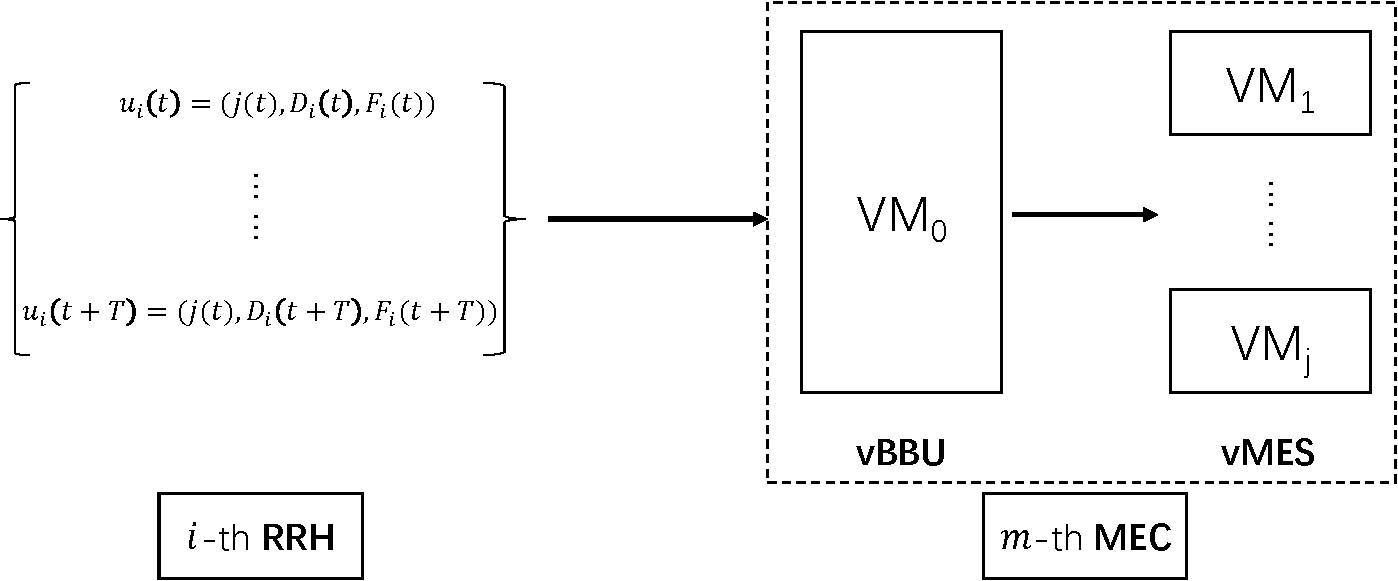
\includegraphics[width=0.9\textwidth]{images/cran-system-model.pdf}
	\caption{The Illustration of System Model.}
	\label{fig:scenario}
\end{figure*}

In this paper, we consider a MEC scenario with C-RAN architecture,
%Based on network function virtualization (NFV), 
where the communication data processing tasks (DTs) and general computation tasks (CTs) can be implemented by virtual BBUs (vBBUs) and virtual MEC servers (vMESs) on general-purposed processors, respectively.
%-----------------------------------------------------------------------------------------%

\section{System Model}
\subsection{Network Model}
There are $I$ RRHs and $M$ edge clouds considered in our network which are denoted as $\mathcal{I}=\set{1,\dots,I}$ and $\mathcal{M}=\set{1,\dots,M}$, respectively.
Each serves the mobile devices (MDs) in its coverage denoted as $\mathcal{C}_{i}$ and has a fronthaul connection to one virtualized BBU (vBBU) in one edge cloud.
Furthermore, we assume that each edge cloud consists of fixed $N$ virtual machines (VMs).

% The time axis of dispatching is organized by time slots.
The system is scheduled with the minimum time unit called \emph{frame}.
In the $t$-th frame, there could be at most one MD in $\mathcal{C}_{i}$ starting to transmit data via the $i$-th RRH to edge clouds $\mathcal{M}$ for further processing.
There are two types of data which would incur two types of tasks, respectively, in the system.
One is called data task (DT), $\dots$, whose average arrival rate is denoted as $\lambda_{0}$.
The other is called computation task (CT), $\dots$, whose average arrival rate is denoted as $\lambda_{j}, \forall j\in\mathcal{J}, \mathcal{J} \define \set{1,\dots,j}$. 
% We use the concept, \emph{active devices}, to name the mobile devices with computation tasks.
% After uplink transmission, DT only need to be assigned vBBU to perform communication computation, while CT needs to be assigned both vBBU and vMES to perform communication computation and service computation.
% The uplink transmission and computation are scheduled in frames, each with duration $T_{\mathrm{F}}$.
% In each frame, there is at most one active mobile device appears in each cell with probability $P_{i}^{\mathrm{N}}$. And the probability that an active device arrived in region $\mathcal{C}'$ is
% \begin{align}
% 	\mathrm{Pr}[\text{New active device in region }\mathcal{C}']=\int_{\mathcal{C}'}\lambda(\mathbf{l})ds(\mathbf{l}),\forall \mathcal{C}'\subset\mathcal{C}_{i}.
% \end{align}
% where $\lambda(\mathbf{l})$ is the probability density of the active device arrived in arbitrary location in the cell region $\mathbf{l}\in\mathcal{C}_{i}$ and $\int_{\mathcal{C}_{i}}\lambda(\mathbf{l})ds(\mathbf{l})=1$. It is assumed that the location of each active device is quasi-static during the period from it arrives to it completes the uplink transmission of the whole task. The active device becomes \textit{inactive} once the edge cloud finishes computing the whole task. Moreover, due to the small data size of the computation output, the downlink latency of the computation output is ignored.
% Let $\mathcal{U}_{i}(t)$ be the set of active devices in the $i$-th cell in $t$-th frame, $\mathcal{D}_{i}(t)\subset\mathcal{U}_{i}(t)$ be the subsets of the active devices whose tasks are just accomplished at the edge cloud in the $t$-th frame, and $n_{i,t}$ be the index of the new active device in the $i$-th cell arrived at the beginning of the $t$-the frame. Therefore, every active device is assigned with a unique index associated with the cell index and frame index it arrived.
% If there is no new active device arrived at the beginning of the $t$-th frame, then $n_{i,t}=\emptyset$. Therefore, the dynamics of the active devices can be represented as
The incurred type-$j$ task in the $i$-th cell in the $t$-th frame is described generally by a tuple $u_{i}(t) \define \big( j(t), D_{i}(t), F_{i}(t) \big)$, where $j(t)$ denotes the job type, $D_{i}(t)$ denotes the input data bits and $F_{i}(t)$ denotes the \emph{deterministic} computation time on the vMESs.
Specifically, the computation time for type-$0$ job (i.e., a data task) has $F_{i}(t)=0$ ($\forall t$).

Let $\rho_{i,\tau}(t)$ denotes the indictor for whether the task appeared in the $\tau$-th frame in the $i$-th cell is in uploading or not.
%FIXME: integrate uploading with above indicator
For uplink transmission, the received signal at the $i$-th RRH from the $n_{i,t}$-th user after receive beamforming is given by
\begin{align}
	y_{i}(t) = \sqrt{p_{i,k}^{\mathrm{Tr}}(t)\rho_{i,i,k}}h_{i,i,k}(t)x_{i,k}(t)+\sum_{(j,m)\neq (i,k)}\sqrt{p_{j,m}^{\mathrm{Tr}}(t)\rho_{i,j,m}}h_{i,j,m}(t)x_{j,m}(t)+z_{i}(t)
\end{align}
where $\sqrt{\rho_{j,i,k}}$ denotes the pathloss from the $(i,k)$-th user to the $j$-th RRH, $h_{j,i,k}(t)\sim \mathcal{CN}(0,\sigma_{j,i,k}^{2})$ denotes the channel gain from the $j$-th RRH to the $(i,k)$-th user.
Then the signal-to-interference-plus-noise ratio (SINR) can be expressed by
\begin{align}
	\gamma_{k}(t)=\frac{p_{i,k}^{\mathrm{Tr}}(t)\rho_{i,i,k}|h_{i,i,k}(t)|^2}{\sum_{(j,m)\neq (i,k)}p_{j,m}^{\mathrm{Tr}}\rho_{i,j,m}|h_{i,j,m}(t)|^{2}+\sigma_{i}^{2}},
\end{align}
Thus, the achievable rate for the $k$-th user is given by
\begin{align}
	r_{k}(t)= W\cdot \text{log}(1+\gamma_{k}(t)), \forall k,
\end{align}
where $W$ is the bandwidth.
The dynamics of the $k$-th transmission queue is given by
\begin{align}
	Q_{k}^{\mathrm{Tr}}(t+1)=(Q_{k}^{\mathrm{Tr}}(t)-D_{k}^{\mathrm{Tr}}(t))^{+}
\end{align}
where $D_{k}^{\mathrm{Tr}}(t)=T_{\mathrm{f}}r_{k}(t)$.
Let ${U}_{i}(t)$ denote the existing tasks in the $i$-th cell in the $t$-th frame
\begin{align}
	\mathcal{U}_{i}(t+1)= \mathcal{U}_{i}(t)\cup\{n_{i,t}\}/\mathcal{D}_{i}(t).
\end{align}

\subsection{Task Computing Models}
Each new active device has a computation-intensive task which needs to be transmitted to the edge cloud for computation. It is assumed that the task of the $k$-th new active device is represented as $u_{k}=(F_{k},D_{k})$, where $F_{k}$ denotes the total number of frames to be completed and $D_{k}$ denotes the total data size of the task input.

The queueing model is illustrated in Fig.1.
The buffer at each active device stores the data packets to be transmitted to its corresponding RRH. The packet size is ${N_\mathrm{b}}$ bits. Then the transmission queue in the $n_{i,t}$-th user and the queue of service computation is given by
\begin{align}
	Q_{n_{i,t}}^{\mathrm{Tr}}(t+1)=\left\lfloor\frac{D_{k}}{N_\mathrm{b}}\right\rfloor,
\end{align}
\begin{align}
	Q_{n_{i,t}}^{\mathrm{C}}(t+1)=F_{k}.
\end{align}

There are two buffers in the edge cloud for each active device. One is the buffer of vBBU pool for communication computation (measured in packets) and the other is the buffer of vMES for service computation (measured in frames), which are denoted as $Q_{k}^{\mathrm{B}}(t)$ and $Q_{k}^{\mathrm{C}}(t)$ respectively.

As in \needref{6582405} and \needref{8353131}, we assume that each server creates $M$ containers and the limited computation capacity of each server is fairly allocated to its hosted containers each with computation resource $f$. The $i$-th container on each server can only perform communication computation or service computation for the tasks of the $i$-th cell. Let the $(s,i)$-th container denotes the $i$-th container on the $s$-th server. The $(s,i)$-th container can be either $\textit{running}$ state or $\textit{shutdown}$ state. When the $(s,i)$-th container is running in a certain frame, it can perform either communication computation or service computation for one certain task of the $i$-th cell. Denote $a_{s,i,k}(t)$ as the binary decision which is $1$ if the $(s,i)$-th container is $\textit{running}$ state for the communication task of the $k$-th task and is $0$ otherwise. Denote $b_{s,i,k}(t)$ as the binary decision which is $1$ if the $(s,i)$-th container is starting to $\textit{running}$ state for service computation of the $k$-th task and $0$ otherwise. As in \cite{}, we assume that the service computation of each task need to be performed in consecutive frames and introduce the binary state $b_{s,i,k}^{-}(t)$ which indicates that the $(s,i)$-th container is still $\textit{running}$ state before the $t$-th frame and $0$ otherwise. Therefore, once $b_{s,i,k}(t)=1$, then $b_{s,i,k}^{-}(t+\tau)=1$, $\tau=1,\ldots,F_{k}-1$.

\begin{align}
	b_{s,i,k}(t)=
	\begin{cases}
		1 &Q_{k}^{\mathrm{Tr}}(t)=0,Q_{k}^{\mathrm{B}}(t)=0,b_{s,i,k}^{-}(t)=0,\text{and container is running state,}\\
		0 &\text{otherwise}.
	\end{cases}
\end{align}

Denote $D_{k}^{\mathrm{B}}(t)$ as the number of packets departing from queue of communication computation which can be given by
\begin{align}
	D_{k}^{\mathrm{B}}(t)=\left\lfloor\frac{T_{\mathrm{f}}f}{\beta^{\mathrm{B}}N_{\mathrm{b}}}\right\rfloor,
\end{align}

Then the queue dynamics are represented as
\begin{align}
	Q_{k}^{\mathrm{B}}(t+1)=(Q_{k}^{\mathrm{B}}(t)-\sum_{s}a_{s,i,k}D_{k}^{\mathrm{B}}(t))^{+}+D_{k}^{\mathrm{Tr}}(t),
\end{align}
\begin{align}
	Q_{k}^{\mathrm{C}}(t+1)=Q_{k}^{\mathrm{C}}(t)-\sum_{s}(b_{s,i,k}(t)+b_{s,i,k}^{-}(t)).
\end{align}

The normalized power consumption of $s$-th physical machine is given by
\begin{align}
	P_{s}(t)= \alpha\left(\frac{\sum_{i}a_{s,i}(t)}{N}\right)^{v}+(1-\alpha)
\end{align}
where $\alpha\in[0,1]$ and $(1-\alpha)$ denotes the normalized power consumption in the idle state for each server.

When both communication computation and service computation of a task is finished, the mobile device becomes $\textit{inactive}$, i.e.,
\begin{align}
	k\in\mathcal{D}_{i}(t),\text{if }Q_{k}^{\mathrm{X}}(t)=0,\mathrm{X}=\mathrm{Tr},\mathrm{B},\mathrm{C}.
\end{align}

\section{Problem Formulation}
The system state in the $t$-th frame is defined by \\
$\mathbf{S}_{t}=\{\rho_{i,j,k},h_{i,j,k}(t),Q_{k}^{\mathrm{Tr}}(t),Q_{k}^{\mathrm{B}}(t),Q_{k}^{\mathrm{C}}(t),a_{s,i}(t),b_{s,i}(t)\}$

The scheduling policy in the $t$-th frame is defined by $\mathbf{\Omega}(\mathbf{S}_{t})=\{p_{i,k}^{\mathrm{Tr}}(t),d_{s,i,k}\}$

The cost function in the $t$-th frame is given by
\begin{align}
	g(\mathbf{S}_{t},\mathbf{\Omega}(\mathbf{S}_{t}))=\sum_{i}|\mathcal{U}_{i}(t)|+\omega_{\mathrm{p}}\bigg(\sum_{i}p_{i,k}^{\mathrm{Tr}}(t)+\sum_{s}p_{s}(t)\bigg)
\end{align}

\begin{align}
	\bar{G}(\mathbf{S},\mathbf{\Omega})=\lim_{T\to\infty}\mathbb{E}_{\{\mathbf{S}_{t}^{\mathrm{N}},\mathcal{H}_{\mathrm{E}}(t)|\forall t\}}\left[\sum_{t=1}^{T}\gamma^{t-1}g(\mathbf{S}_{t},\mathbf{\Omega}(\mathbf{S}_{t}))|\mathbf{S}_{1}=\mathbf{S}\right]
\end{align}

\begin{align}
	\mathbf{\Omega}^{*}=\mathop{\arg\min}_{\mathbf{\Omega}}\bar{G}(\mathbf{S},\mathbf{\Omega})
\end{align}

\begin{align}
	V(\mathbf{S}_{t})=\min_{\mathbf{\Omega}(\mathbf{S}_{t})}\left[g(\mathbf{S}_{t},\mathbf{\Omega}(\mathbf{S}_{t}))+\sum_{\mathbf{S}_{t+1}}\gamma\Pr(\mathbf{S}_{t+1}|\mathbf{S}_{t},\mathbf{\Omega}(\mathbf{S}_{t}))V(\mathbf{S}_{t+1})\right]
\end{align}


\appendices
\bibliographystyle{IEEEtran}
\bibliography{C-RAN_and_MEC}



\end{document}


